\chapter{Theoretical framework}\label{ch:3}


\section{The mathematical model} \label{sec:modelo}

To describe the thermoluminescent response of a semiconductor, we can use a mathematical model based on the trapping and releasing of charge carriers in the accessible energy levels of the material. 

\vspace{10pt}

Let us first consider the case of an arbitrary semiconductor without impurities. The energy levels of the conduction band and the valence band are separated by a bandgap $E_g$, and can be obtained with Schrodinger's equation that is under the influence of a periodic potential:

\begin{equation} \label{eq:schrodinger}
  \left[ -\frac{\hbar^2}{2m} \nabla^2 + V(\vec{r}) \right] \psi(\vec{r}) = E ~ \psi(\vec{r}),
\end{equation}

\vspace{10pt}
The periodicity of the potential $V(\vec{r})$ for any lattice vector $\vec{R}$ allows the Bloch's theorem to apply, and so it gives rise to the formation of a band structure, composed by the valence band, which is typically fully occupied at absolute zero temperature, and the conduction band, which is in turn typically empty -or rather, we can consider it filled with holes ($h^+$), or ``positively charged electrons''. The bandgap $E_g$ is then defined as the energy difference between the top of the valence band and the bottom of the conduction band, and for a perfect crystal, no energy states are allowed in that region. This can be clearly seen if we take into account the density of available states, $D(E)$, which is a function of the Fermi-Dirac distribution $f(E)$ for a certain temperature $T$. This function gives the occupancy of any energy level $E$, and can be expressed as:

\begin{equation} \label{eq:fermidirac}
  f(E) = \frac{1}{e^{\frac{E - E_f}{k_B T}} + 1},
\end{equation}

\vspace{10pt}
Where $E_f$ is the Fermi Level, and $k_B$ is the Boltzmann constant. If the system is in equilibrium, and we set the case of $T=0K$, the occupancy function $f(E)$ will be equal to 1 for all energy levels below the Fermi level, and 0 for all energy levels above it. This means that the occupancy function will be a step function, with a discontinuity at the Fermi level, and so we can see that there are no available states in the bandgap region.

\begin{figure}
  \centering
  
\includegraphics[width=\textwidth]{Images/FD_irradiation.png}
  \caption[Fermi-Dirac distributions at different temperatures and TL process stages.]{Fermi-Dirac distribution $f(E)$ plotted against energy for different temperatures (0.1 K, 300 K and 600 K) at four key stages of the thermoluminescence process: (a) Before irradiation, where electrons follow a standard Fermi-Dirac distribution centered at the Fermi Level $E_F$; (b) After irradiation, the systems develops separate quasi-Fermi levels for electrons ($E_{Fe}$) and holes ($E_{Fh}$), deforming the previous distribution; (c) During stimulation, where thermal effects shift both quasi-Fermi levels closer to equilibrium, and the distribution approaches the original shape; (d) Final equilibrium, where the system returns to a standard Fermi-Dirac distribution with the Fermi Level $E_F$ restored. }
  \label{fig:FD_irradiation}
\end{figure}

\begin{figure}[H]
  \centering
  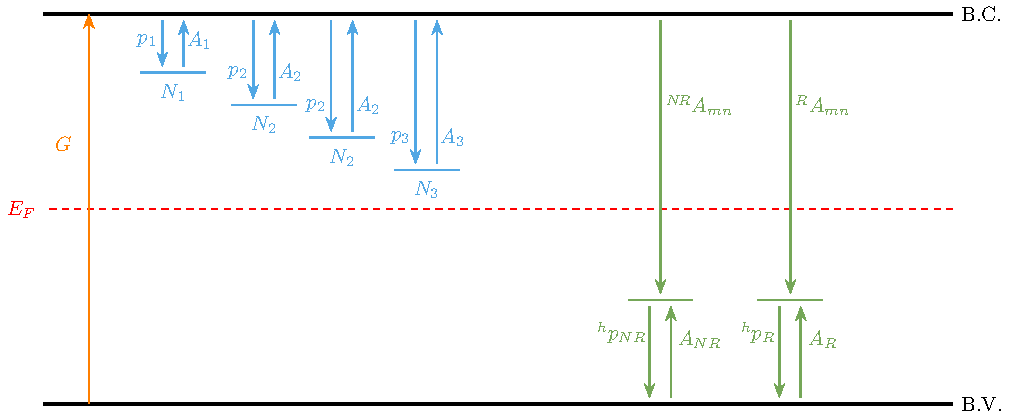
\includegraphics[width=\textwidth]{Images/modeldiagram.pdf}
  \caption[Jab\l oński diagram illustrating the theoretical TL model with traps and transitions.]{Jab\l oński diagram of the theoretical model for the thermoluminescence process. The energy is situated in the Y axis, and the different components of the system are shown: traps ($p_k$: electron release probability, $A_k$: recombination probability, $N_k$: total density of available positions), recombination centers ($^hp_j$: hole excitation probability, $A_j$: electron trapping probability, $^jA_{mn}$: electron recombination probability), and the conduction (C.B) and valence (V.B) bands with the respective electron-hole pair generation rate ($G$).}
  \label{fig:TheoreticalModel}
\end{figure}

\vspace{10pt}
The introduction of impurities or defects however, break the periodicity of the lattice, and create localized energy levels inside this ``forbidden region''. These levels can be thought of as traps for electrons if we are situated above the fermi level, and traps of holes if we are situated below. When this material is irradiated, electrons from the valence band can be excited to the conduction band, creating an electron-hole pair; and so changing the shape of the occupancy function. Once excited, both electrons and holes get ``trapped'' in these localized energy levels, and the excitation of these pairs into equilibrium will result in the emission of energy. In Figure \ref{fig:FD_irradiation} we can see a broad description of the perturbation of the system from its equilibrium state due to the irradiation, and the return of the system to equilibrium during either thermal stimulation or optical stimulation. If said relaxation processes are radiative, TL and OSL result. 

\vspace{10pt}

And so, we can see a schematic representation of our theoretical model in Figure \ref{fig:TheoreticalModel}. Situating the energy in the Y axis, the focus is set in the energy gap of our material. Drawn as a blue or green horizontal line are the energy traps; in blue above the Fermi level there are electron traps, and in green there are ``hole traps'' or recombination centers. The vertical arrows describe available transitions; the ones pointing upwards represent an excitation process, and the ones pointing downwards represent a relaxation process. 

\vspace{10pt}

Mathematically, we can describe these processes with a set of differential equations that take into account the rate of change of the number of electrons and holes in the bands and traps. This set will depend on the properties of the material, and the luminescence response we are trying to model. For an arbitrary system, we can write the following set of equations that describe the rate of change of the number of electrons and holes in the conduction band $n_c$, the valence band $n_v$:
\vspace{10pt}

\begin{equation} \label{eq:dn_cdt}
  \frac{dn_c}{dt} = \textcolor{orange}{G} - \textcolor{customblue}{\left[\sum_i \frac{dn_i}{dt}\right]} \cdot n_c - \textcolor{customgreen}{\left[ \sum_{j=R, N\!R}\, ^jA_{mn} \cdot m_j \right]} \cdot n_c
\end{equation}

\begin{equation} \label{eq:dn_idt}
  \textcolor{customblue}{\frac{dn_i}{dt} = -p_i \cdot n_i + A_i \cdot [N_i - n_i]}
\end{equation}

\begin{equation} \label{eq:dm_jdt}
  \textcolor{customgreen}{\frac{dm_j}{dt} = -^hp_j \cdot m_j + A_j \cdot [M_j - m_j]} \cdot n_v - \textcolor{customgreen}{^iA_{mn} \cdot m_j} \cdot n_c
\end{equation}

\begin{equation} \label{eq:dn_vdt}
  \frac{dn_v}{dt} = \textcolor{orange}{G} - \textcolor{customgreen}{\sum_{j=R, N\!R} \left[-^hp_j \cdot m_j + A_j \cdot [M_j - mj] \textcolor{black}{~ \cdot ~n_v}\right]} 
\end{equation}

\vspace{15pt}
Where every term is defined as follows:
\begin{itemize}[itemsep=0.2cm,parsep=0cm]
  \item $G$: electron-hole pairs generation rate by the radiation [cm$^{-3}$ s$^{-1}$]
  \item $n_c$: electron concentration in the conduction band [cm$^{-3}$]
  \item $n_v$: electron concentration in the valence band [cm$^{-3}$]
  \item $n_i$: electron concentration in trap i [cm$^{-3}$]
  \item $m_j$: hole concentration in the recombination center j [cm$^{-3}$]
  \item $N_i$: total density of available positions in trap i [cm$^{-3}$]
  \item $M_j$: total density of available positions in recombination center j [cm$^{-3}$]
  \item $p_i$: electron release probability factor for trap i [s$^{-1}$]
  \item $^hp_j$: hole release probability factor for recombination center j [s$^{-1}$]
  \item $A_i$: electron trapping probability factor for trap i [cm$^{3}$ s$^{-1}$]
  \item $^jA_{mn}$: recombination probability factor for recombination center j [cm$^{3}$ s$^{-1}$]
\end{itemize}

\vspace{10pt}

Equation \ref{eq:dn_cdt} describes the change rate of electron concentrations in the conduction band. To interpret this equation, we can see that to the electron-hole pairs generated by the radiation ($G$), there are two terms subtracted. The first one correlates to the electrons that leave the continuum levels of the conduction band and get trapped in the discrete levels of the material ---a process described by \ref{eq:dn_idt}, that will have a further discussion in section \ref{sec:factorfrecuencia}---, and the second one answers to the electrons in the conduction band that recombine with holes with a radiative ($R$) or non-radiative ($N\!R$) process. It is easy to see that this second term corresponds to the third term of \ref{eq:dm_jdt}. 

\vspace{10pt}
The change rate of electron concentrations in the valence band is shown in \ref{eq:dn_vdt}, and it follows a similar logic. This time however, we only take into account the terms multiplied by the electron density in the valence band ($n_v$) seen in equation \ref{eq:dm_jdt}; one that represents the holes leaving the continuum to get trapped in the recombination centers, and another that accounts for the addition of electrons that are released from the recombination centers and recombine with the holes in the valence band. The terms described correspond to Equations \ref{eq:dn_idt} and \ref{eq:dm_jdt} describe the total change rate of electrons and holes in the discrete levels of the material. The signs of the terms in these equations follow the convention that we are set in the conduction band, and so any electron that leaves the conduction band is represented with a negative term, and any electron that enters is represented with a positive term.

\vspace{10pt}

To carry out a numerical simulation of the process, we will need to solve the set of differential equations \ref{eq:dn_cdt} -- \ref{eq:dn_vdt} using RKF-45 method, which is a Runge-Kutta method of order 4 and 5. This method will obtain the charge concentration in all traps and recombination centers at an instant of time. The solving of this set of equations will be done for the three phases required to obtain the TL glow curve. To do this, the intrinsic and kinetic parameters are kept constant, varying the external conditions of the system such as temperature and electron-hole pair generation rate. 

\vspace{10pt}
The first phase is \textit{irradiation}, where the material is exposed to ionizing radiation. It begins with all levels initially empty [$n_c(0) = n_v(0) = n_i(0) = m_j(0) = 0$], and the electron-hole pairs generated as a result will have a constant value as a function of time ($G = 1000$ cm$^{-3}$ s$^{-1}$). The temperature is set to a constant $T = 25$ \textdegree C and the filling process takes one hour (3600 seconds). The second phase is \textit{relaxation}, where the material is left undisturbed at a constant temperature for a defined period of time. Taking as initial values the final values of the irradiation phase, the temperature is kept constant at $T = 25$ \textdegree C, and the electron-hole pairs generation rate is set to $G = 0$ cm$^{-3}$ s$^{-1}$. The relaxation process is set for one week (604,800 seconds). Finally, the third phase is \textit{heating}, where the material is taken from an initial temperature $T_0$ to a final temperature at a constant linear heating rate during 400 seconds. The numerical resolution of the set equations is similar to the previous phases, but now with the temperature varying linearly with the expression:

\begin{equation} \label{eq:heating}
  T(t) = T_0 + \beta \cdot t
\end{equation}

\vspace{7pt}
Where the heating rate is set to $\beta = 1 $ \textdegree C s$^{-1}$. The electron-hole pairs generation rate is set to $G = 0$ cm$^{-3}$ s$^{-1}$, and the charge concentration values are taken from the final values of the relaxation phase. The heating process is set to last 400 seconds. The results after the numerical resolution of the set of equations will be the charge concentration values for every instant of time throughout the whole heating cycle [$n_c(t), n_v(t), n_i(t), m_j(t)$]. It is in this phase when the luminescent emission occurs, and so the intensity of the emitted light can be estimated in relation to the radiative recombination of electron-hole pairs. We can give the expression for the intensity of the emitted light as it follows:

\begin{equation} \label{eq:intensity}
  I_{T\!L}(t) = -\frac{dm}{dt} \approx {}^RA_{mn} \cdot m_R \cdot n_c
\end{equation}

\vspace{7pt}

We can write this dependence as a function of temperature by:

\begin{equation}
  I_{T\!L}(t) = -\frac{dm}{dt} = -\frac{dm}{dt} \cdot \frac{dT}{dT} = -\frac{dm}{dT} \cdot \frac{dT}{dt} = -\frac{dm}{dT} \cdot \beta = I_{T\!L}(T) \cdot \beta
\end{equation}

Representing this intensity as a function of temperature will be the objective of the simulations, as it is the key to understand the thermoluminescent response of the LiF:Mg,Ti after being irradiated.

\section{Analysis of the electron release probability} \label{sec:factorfrecuencia}

As introduced in Section \ref{sec:modelo}, there is a greater discussion to be had about the releasing probability of electrons and holes, as it determines in great part the electron-hole pairs available to recombine. In general, two distinct mechanisms may contribute to the release of a trapped carrier: \textit{thermal} and \textit{optical (photo)excitation}. In the first one, the electron gains sufficient energy from lattice vibrations to overcome the trap depth, and in the latter the release is induced by the absorption of a photon whose energy exceeds the one binding the carrier to the trap. An electron trapped in a lattice defect with energy $E_t$ and temperature $T$ will have a probability of being released that is the result of:

\begin{equation}
  p = p_{th} + p_{ph}
\end{equation}

Where $p_{th}$ is the thermal excitation probability and $p_{ph}$ is the optical excitation probability. The thermal contribution follows Arrhenius equation. The probability per unit of time that the electron will be thermally excited into the conduction band is given by:

\begin{equation} \label{eq:p_th}
  p_{th} = s \cdot e^{-\frac{E_t}{k_B T}}
\end{equation}

\vspace{10pt}
Where $s$ is known as the \textit{frequency factor} [s$^{-1}$]. It can be interpreted as the ``attempt to escape'' frequency, as it is a measure of the number of times per second that energy is absorbed from phonons in the lattice. The exponential that follows is the probability that the energy absorbed is enough to cause a transition from the localized state to the conduction band. For the optical contribution on the other hand, the trapped electrons are released from their traps via absorption of energy from photons \cite{mckeever_course_2022}, and the probability is given by:

\begin{equation}
  p_{\text{ph}} = \sigma_P(E) \cdot \Phi
\end{equation}

Where $\sigma_P(E)$ is the photoionization cross-section [cm$^2$], which is a measure of the probability that a photon with energy $E$ will be absorbed by an electron trapped in a lattice defect, and $\Phi$ is the photon flux or intensity of the stimulating light [cm$^{-2}$ s$^{-1}$], which is the number of photons per unit area per unit time. This process is particularly relevant in optically stimulated luminescence (OSL), where the material is stimulated with light to release the trapped electrons and produce a luminescent signal. If $E_0$ is the threshold photon energy required to excite the electron from the trap, instead of considering only the thermal trap depth $E_t$ as one may expect, we should initially consider the effect of the contribution of lattice phonons such that:

\begin{equation}
  E_0 = E_t + E_{ph}
\end{equation}

Where $E_{ph}$ is given by:

\begin{equation}
  E_{ph} = S_{H\!R} \cdot h \cdot \nu_{ph}
\end{equation}

\vspace{7pt}

And here $S$ is the Huang-Rhys factor, which is a dimensionless parameter that characterizes the degree of electron-phonon coupling in a luminescent material that usually ranges on the order of 1--2 \cite{mckeever_1995}. The higher the Huang-Rhys factor, the stronger the electron-phonon coupling, and so the greater the energy shift of the trap level due to lattice vibrations. The term $h \cdot \nu_{ph}$ is the phonon energy with frequency $\nu_{ph}$ [s$^{-1}$], where $h$ is Planck's constant [eV $\cdot$ s]. For LiF the phonon frequency is typically around 900 cm$^{-1}$ \cite{bransden_atomics}, which corresponds to a phonon energy of approximately 0.11 eV. If we take a Huang-Rhys factor of $S_{HR} = 1$, we can estimate the energy shift given a set of experimental values for the thermal energies $E_t$ of the traps. The results are shown in \ref{tab:energythresholds} and with them we see that the energy threshold $E_0$ is primarily determined by the thermal trap depth $E_t$, with the phonon energy $E_{ph}$ contributing a small correction.

\renewcommand{\arraystretch}{1.5}
\begin{longtable}[c]{lllll}
\caption[Energies for the different traps and recombination centers in LiF:Mg,Ti.]{Energies for the different traps and recombination centers in LiF:Mg,Ti. $E_t$ represents the thermal energy, $E_{ph}$ the phonon energy, and $E_0$ the total energy threshold.}
\label{tab:energythresholds}\\
\hline
\multicolumn{2}{l}{Parameters}                            & $E_t$ (eV) & $E_{ph}$ (eV) & $E_0$ (eV) \\ \hline
\endhead
\hline
\endfoot
\endlastfoot
\multirow{6}{*}{Trapping Centers}      & Trap I        & 1.19       & 0.11         & 1.30       \\
                                       & Trap II       & 1.60       & 0.11         & 1.71       \\
                                       & Trap III      & 1.76       & 0.11         & 1.87       \\
                                       & Trap IV       & 1.87       & 0.11         & 1.98       \\
                                       & Trap V        & 1.98       & 0.11         & 2.09       \\
                                       & Trap s        & 2.70       & 0.11         & 2.81       \\ \hline
\multirow{2}{*}{Recombination centers} & Radiative     & 2.30       & 0.11         & 2.41       \\
                                       & Non Radiative & 2.30       & 0.11         & 2.41       \\ \hline
\end{longtable}

\vspace{10pt}

This observation reinforces the suitability of studying the TL independently of optically stimulated luminescence (OSL). The fact that the thermal energy $E_t$ stays over zero confirms that thermal energy alone is sufficient to release charge carriers from traps over a physically accessible temperature range. Furthermore, in TL measurements, no external optical stimulation is applied during readout, and so the photon flux in a darkened environment is negligible. As a result, photo-induced excitation does not contribute meaningfully to the observed luminescence signal. From now on, we will close our focus on the thermoluminescence process, and so we will only consider the thermal excitation probability $p_{th}$ in our simulations.

\vspace{10pt}

If we aim to deepen our understanding of equation \ref{eq:p_th}, we can look a little further in the concept of the frequency factor $s$. It is a crucial parameter in the study of thermoluminescence, as it determines the rate at which electrons are released from traps. It is a function of the material properties, as shown in its definition:

\begin{equation} \label{eq:freqfactor}
  s = \nu_{ph} \cdot K \cdot e^{\frac{\Delta S}{k_B}}
\end{equation}

\vspace{10pt}
Where $\nu_{ph}$ is the lattice phonon vibration frequency and $K$ is the transition probability constant, that takes the value 0 or 1 depending on whether the transition is allowed or forbidden. Typically, one can expect $s \sim 10^{12} -10^{14}$ s$^{-1}$, which is consistent with the values of $\nu$ for most solids. The term $e^{\nicefrac{\Delta S}{k_B}}$ is a correction factor that accounts for the entropy change associated with the transition from the localized state to the conduction band. 

\vspace{10pt}

From equation \ref{eq:freqfactor} we see that the frequency factor has an exponential dependency with the entropy change. This, taking the Quantum Statistical Mechanics theory \cite{brey}, does not align with the invariance of said factor with temperature, as entropy, with its own definition, should vary when temperature does. While a rigorous proof of the overall temperature dependence of the frequency factor is beyond the scope of this work, one model is proposed to provide an approximate perspective on how this dependency could influence the resulting TL glow curve. 

\vspace{10pt}

At first glance, the simplest model was considered, where the entropy would be linear with the temperature ($\Delta S \propto T$). This theory was quickly discarded as would make the entropy factor increase exponentially with the temperature ($s \propto e^T$), and so the probability of excitation would tend to infinity in a very short range of temperature increase.

\vspace{10pt}

To solve this issue, a more refined model was considered, where the entropy would now be logarithmically dependent on the temperature ($\Delta S \propto \ln(T)$). The constant of the proportionality could be called $\alpha$, and so the resulting expression of the frequency factor can be written as:

\begin{equation}\label{eq:freqfactor_lnT}
    s = \nu_{ph} \cdot K \cdot T^{\nicefrac{\alpha}{k_B}}
\end{equation}

\vspace{10pt}

It is clear now that a softer dependency with the temperature is achieved, and the previous problem of the entropy factor tending to infinity is solved. The value of $\alpha$ can be adjusted to keep the entropy contribution at a realistic magnitude ---typically we have $\Delta S \sim  1\!-\!3 ~~k_B$ over the glow curve temperature range---. For that reason, we have selected a value of:

\begin{equation}
    \alpha = \frac{1.5 ~k_B}{ln(300)} \approx 0.26 ~k_B
\end{equation}

\vspace{10pt}

This choice ensures that the frequency factor remains within a reasonable range across the temperature spectrum of interest, and yields TL glow curves that are consistent with experimental observations of LiF:Mg,Ti materials.


\section{About LiF:Mg,Ti} \label{sec:LiF}


Lithium fluoride (LiF) is a crystalline material that has been widely used in radiation dosimetry due to its favorable % !!!!
properties. It first appeared as a thermoluminescent dosimetry material in the 1950's, and since then, it has been extensively studied in the field of radiation detection. The material is composed of lithium (Li) and fluor (F) %?????
atoms, forming a crystal lattice structure of a face-centered cubic (FCC) type. Without any impurities, LiF is a semiconductor, with a bandgap of approximately 14 eV, which makes it an excellent insulator at room temperature.

\vspace{10pt}

To enhance the properties for radiation detection, LiF is often doped with magnesium (Mg) and titanium (Ti) ions, and sold commercially as TLD-100 \cite{horowitz_thermoluminescence_2007}. The doping process introduces defects in the crystal lattice, creating energy levels within the bandgap. These defects play a crucial role in trapping and releasing charge carriers, which are responsible for the thermoluminescent response of the material. This process is known as thermoluminescence, where the trapped electrons are released upon heating, resulting in the emission of light. The intensity of this emitted light is proportional to the amount of radiation absorbed by the material, making it a valuable tool for dosimetry.

\vspace{10pt}

The TL response of LiF:Mg,Ti is characterized by a glow curve, which is a plot of the intensity of emitted light as a function of temperature. The glow curve typically exhibits several peaks, each corresponding to different trapping levels in the material. The position and shape of these peaks can provide valuable information about the trapping and recombination processes occurring in the material, and they are key to understanding the thermoluminescent response of LiF:Mg,Ti. In Figure \ref{fig:ExperimentalGlowCurve} we can see an experimental glow curve of LiF:Mg,Ti plotted with data provided by the Radiation Dosimetry Laboratory of CIEMAT, which shows a typical response with several peaks at different temperatures. 

\begin{figure}[ht]
    \centering
    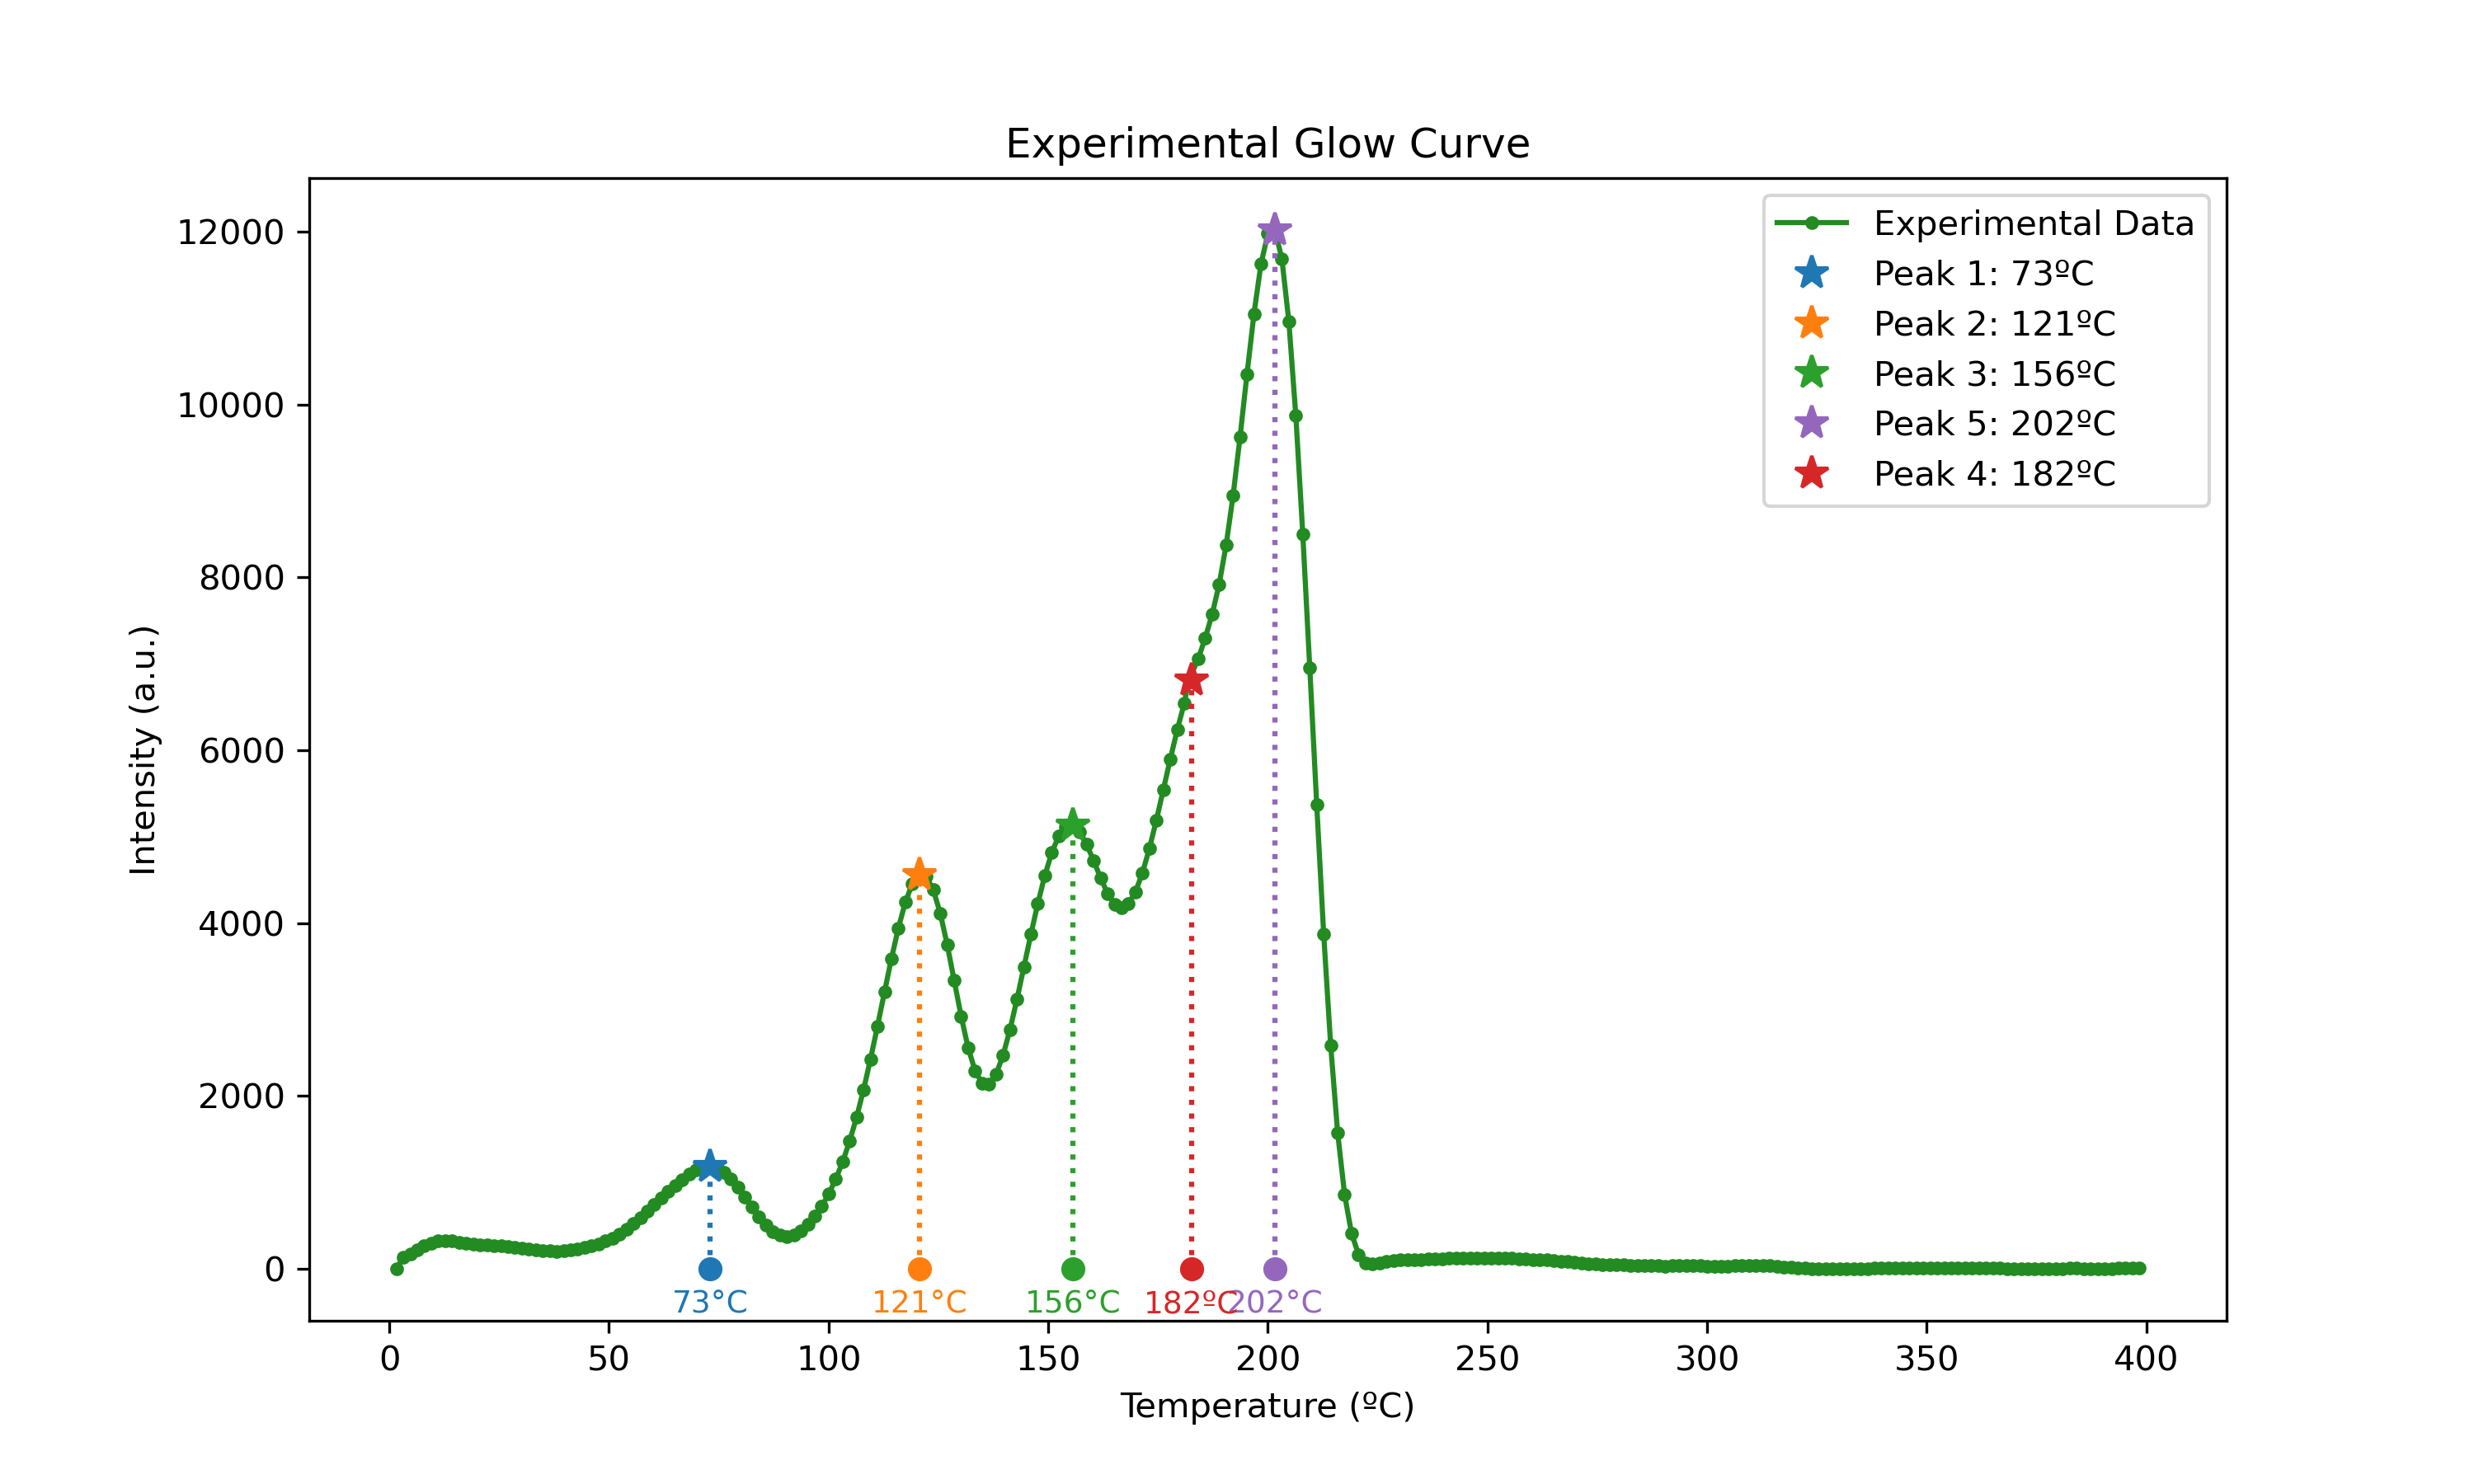
\includegraphics[width=\textwidth]{Images/Experimental_Glow_Curve.png}
    \caption[Experimental TL glow curve of LiF:Mg,Ti.]{Experimental thermoluminescence glow curve of LiF:Mg,Ti showing the emitted light intensity [u.a] plotted against temperature (\textdegree C). The most prominent is the main dosimetric peak around 200 \textdegree C, which is stable and reproducible. Lower-temperature peaks (<150 \textdegree C) correspond to shallow traps with poor thermal stability, while intermediate peaks (150–200 \textdegree C) suggest more complex trapping mechanisms. The measurement reflects the material’s characteristic response following exposure to ionizing radiation.}
    \label{fig:ExperimentalGlowCurve}
\end{figure}
\vspace{10pt}

This characteristic shape of the glow curve for LiF:Mg,Ti has been extensively documented \cite{mckeever_course_2022} \cite{benavente_LiF} \cite{massillon-jl_role_nodate}, and it is a result of the specific energy levels introduced by the doping process, with the main peak typically occurring around 200 \textdegree C. Each peak arises from the thermal release of electrons from traps of different activation energies, if followed by recombination in the recombination centers. The graph shows the luminescence intensity plotted against temperature, and reveals five distinct glow peaks. Each of those peaks corresponds to the thermal release of trapped charge carriers from specific trap levels, and their height and position can be crucial to determine the trap depth and recombination probability. They can be categorized into:

\begin{itemize}
  \item \textbf{Main dosimetric peak ($\sim$ 200 \textdegree C).} It has the most favorable characteristics for dosimetry: high intensity, good linearity with dose, and appears consistency at the same temperature, which helps to exhibit good reproducibility across different measurements and a relatively simple kinetic behavior. It is thermally stable at room temperature for long periods of time, meaning their signal do not fade significantly over days or weeks. 
  \item \textbf{Lower-temperature peaks (< 150 \textdegree C).} They are associated with shallower traps, and are thermally less stable at ambient conditions. They tend to fade significantly at room temperature over time ---that is, undergo great signal loss due to thermal stimulation from room temperature alone---, and as a consequence, are not useful for dosimetric purposes. However, they are useful for fundamental studies of trapping and recombination processes, offering insight into the energy structure of the material and their mechanisms of carrier release. 
  \item \textbf{Intermediate peaks (between 150 \textdegree C and 200 \textdegree C).} As expected, they suppose a middle ground. These peaks represent a transitional region in trap stability and interaction complexity. They are believed to arise from more complex or composite trapping structures, possibly involving multiple trapping levels or interactions between traps and recombination centers and their intensity and position can shift or merge depending on the specific conditions of the sample, the dose or the thermal history. In some cases, peaks in this range can interfere with or overlap the main dosimetric peak, which can complicate deconvolution and dose evaluation.
\end{itemize}
